\documentclass{article}
\usepackage[a4paper,left=10mm,right=10mm,top=15mm,bottom=15mm]{geometry}
\usepackage{amssymb,amsthm,latexsym,amsfonts, amsmath, bm}
\usepackage[lined,ruled]{algorithm2e}
\usepackage{extarrows}
\usepackage{enumerate}
\usepackage{tikz}
\usepackage{underoverlap}
\usepackage{colortbl}
\usepackage{graphicx}
\usepackage{float}
\newtheorem*{lemma}{Lemma}
\newtheorem{theorem}{Theorem}
\title{Exercises for Algorithmic Bioinformatics II\\
Assignment 8}
\author{Xiheng He}
\date{December 2021}
\linespread{2.0}
\begin{document}
\flushright{Wintersemester 2021/22}
\flushleft{Xiheng He}
\flushleft{Lisanne Friedrich}
{\let\newpage\relax\maketitle}
\begin{flushleft}
\textbf{Exercise 4 (ClustalO \& ClustalW, 10P):}
\newline
Read the following publication on the multiple sequence alignment algorithm Clustal Omega:
\newline
Sievers, Fabian, and Desmond G. Higgins. \textit{Clustal Omega for making accurate alignments of many protein sequences.} Protein Science 27.1 (2018): 135-145.
\newline
Apply both algorithms (ClustalO + ClustalW) to the sequences below. Visualize and discuss the
resulting MSA appropriately:
\newline \\
\texttt{Human: TAVCMECFREAAYTKRLGTEKEVEVIGGADKYHSVCRLCYFKKA} \\
\texttt{Danio Rerio: NAVCMQCFKEAAYTKRLGAEKEVEVIGGSDKYHAVCRCCY} \\
\texttt{Tryp Brucei: SAVCMECHNRKASFTYRTVKSDERKLVGGSDMYMSVCRSCYETK} \\
\texttt{Mus Musc: TAVCMECFREAAYTKRLGLEKEVEVIGGADKYHSVCRLCYFKKS} \\
\texttt{Vac Virus: TAVCMKCFKEASFSKRLGEETEIEIIGGNDMYQSVCRKCY} \\
\texttt{Leishm Major: TAVCMMCHEQPACFTRRTVNVEQQELIGGADMYIATCRECYSKQ} \\
\texttt{Thermot Marit: AVCHRCGEYNATLTLKVAGGEEEIDVGGQEKYIAVCRDCY} \\
\texttt{Human M163: TAVCMECFREAAYSKRLGTEKEVEVIGGADKYHSVCRLCYFKKA}
\newline \\
For extra points: compare and discuss the ClustalO/ClustalW MSA with the result of your center-star implementation!
\begin{itemize}
    \item In a nutshell: 
    \newline
    ClustalW is a matrix-based algorithm where Clustal Omega is consistency-based.
    They both use pairwise alignments like EMBOSS and LALIGN, but ClustalW use similarity for MSA where Clustal Omega uses
    seeded guide trees and a new HMM engine that focuses on two profiles to generate MSA.
    \item Algorithm: \begin{itemize}
        \item ClustalW:
        \newline
        ClustalW uses progressive alignment methods as stated above. 
        In these, the sequences with the best alignment score are aligned first, 
        then progressively more distant groups of sequences are aligned. 
        This heuristic approach is necessary due to the time and memory demand of finding the global optimal solution. 
        The first step to the algorithm is computing a rough distance matrix between each pair of sequences, 
        also known as pairwise sequence alignment. The next step is a neighbor-joining method that uses midpoint rooting to create an overall guide tree. 
        The process it uses to do this is shown in the detailed diagram for the method to the right. The guide tree is then used as a rough template to generate a global alignment.
        \item ClustalO: 
        \newline
        Clustal Omega has five main steps in order to generate the multiple sequence alignment. 
        The first is producing a pairwise alignment using the k-tuple method, also known as the word method. 
        This, in summary, is a heuristic method that isn't guaranteed to find an optimal alignment solution, 
        but is significantly more efficient than the dynamic programming method of alignment. 
        After that, the sequences are clustered using the modified mBed method. The mBed method calculates pairwise distance using sequence embedding. 
        This step is followed by the k-means clustering method. Next, the guide tree is constructed using the UPGMA method. 
        This is shown as multiple guide tree steps leading into one final guide tree construction because of the way the UPGMA algorithm works. 
        At each step, (each diamond in the flowchart) the nearest two clusters are combined and is repeated until the final tree can be assessed. 
        In the final step, the multiple sequence alignment is produced using HHAlign package from the HH-Suite, which uses two profile HMM's. 
        A profile HMM is a linear state machine consisting of a series of nodes, each of which corresponds roughly to a position (column) in the alignment from which it was built.
    \end{itemize}
    \item Time complexity: 
    \newline
    ClustalW : $\Omega(N^2)$, ClustalO : $\Omega(L^N)$ ($L$ is the length of the alignment, $N$ is the number of sequences)
\end{itemize}
\begin{figure}[H]
    \centering
    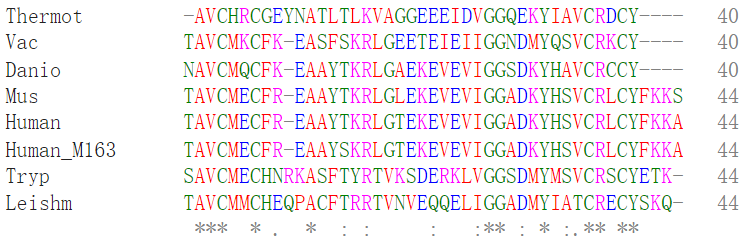
\includegraphics[scale=0.8]{alignment.png}
    \caption{mutiple sequence alignment}
\end{figure}
\begin{figure}[H]
    \centering
    \includegraphics[scale=0.6]{tree.png}
    \caption{phylogenetic tree}
\end{figure}
\end{flushleft}
\end{document}